\newpage
\section{Conclusions}
\subsection{Realistic System Simulation}
\label{subsec:realistic_system_simulation}
A seguito delle analisi descritte nel paragrafo precedente, ho voluto integrare il progetto con una simulazione grafica reale, per dimostrare che la simulazione è corretta.

\noindent
I parametri della simulazione reale utilizzati sono:

\begin{itemize}
    \item $nstep = 100'000$
    \item $step = 250$
    \item $ni = 100$
    \item $nj = 100$
    \item $tfac = 0.01f$
    \item $size = ni \times nj = 10'000$
\end{itemize}

\begin{figure}[htbp]
    \centering

    % Row 1
    \begin{subfigure}[b]{0.48\textwidth}
        \centering
        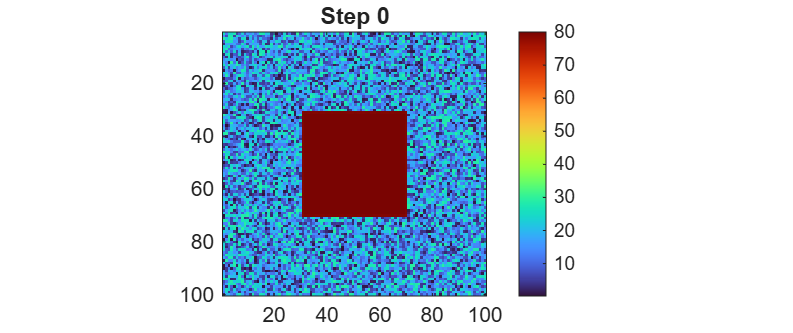
\includegraphics[width=\textwidth]{assets/conclusions/img1.png}
    \end{subfigure}
    \hfill
    \begin{subfigure}[b]{0.48\textwidth}
        \centering
        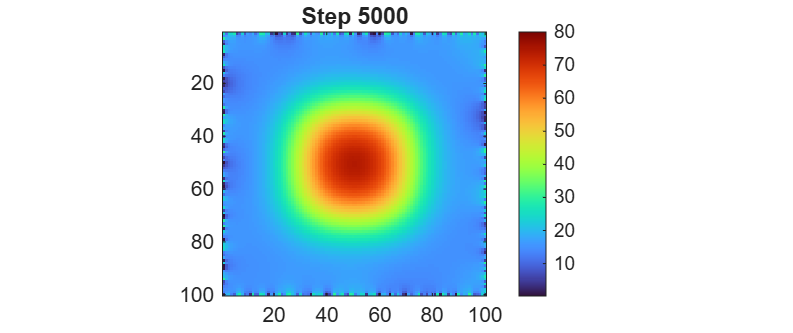
\includegraphics[width=\textwidth]{assets/conclusions/img2.png}
    \end{subfigure}

    \vspace{0.6cm}

    % Row 2
    \begin{subfigure}[b]{0.48\textwidth}
        \centering
        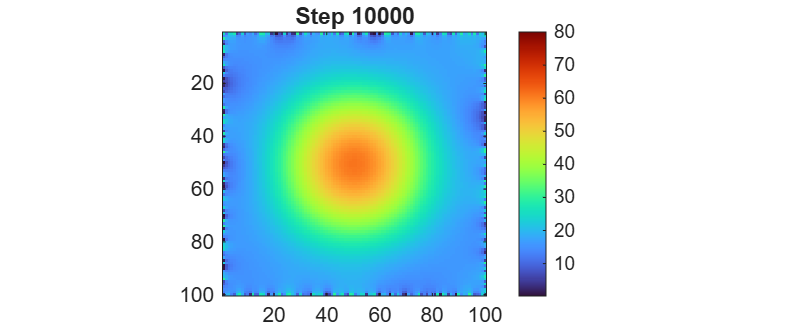
\includegraphics[width=\textwidth]{assets/conclusions/img3.png}
    \end{subfigure}
    \hfill
    \begin{subfigure}[b]{0.48\textwidth}
        \centering
        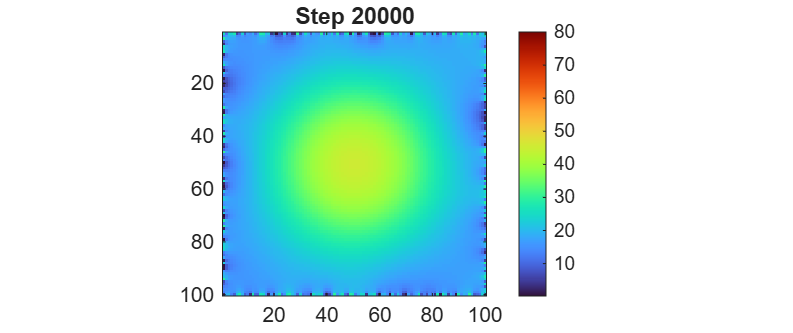
\includegraphics[width=\textwidth]{assets/conclusions/img4.png}
    \end{subfigure}

    \vspace{0.6cm}

    % Row 3
    \begin{subfigure}[b]{0.48\textwidth}
        \centering
        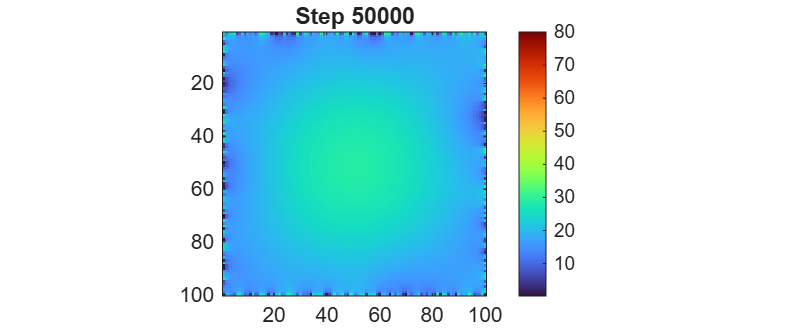
\includegraphics[width=\textwidth]{assets/conclusions/img5.png}
    \end{subfigure}
    \hfill
    \begin{subfigure}[b]{0.48\textwidth}
        \centering
        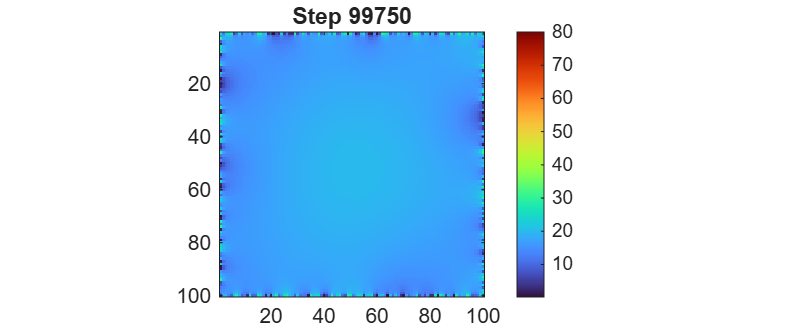
\includegraphics[width=\textwidth]{assets/conclusions/img6.png}
    \end{subfigure}
\end{figure}

\newpage
\subsection{Considerations}
La parallelizzazione tramite GPU ha permesso di ottenere uno speedup significativo, dimostrando l'efficacia dell'approccio rispetto alla CPU.\\

\noindent
L'errore massimo tra GPU e CPU è stato calcolato per verificare la correttezza dei risultati. Nella simulazione corrente, il massimo errore osservato era entro i limiti accettabili (0.0005).\\

\noindent
I risultati confermano che la parallelizzazione con CUDA riduce significativamente i tempi di esecuzione rispetto alla versione sequenziale, mantenendo la precisione numerica.